\chapter{Structuring Arrays with Algebraic Shapes}
\label{star}

\textbf{Array programming} is a programming paradigm focusing on arrays as a fundamental data structure, stemming from Iverson's \emph{array programming model} \cite{apl}. It plays a key role in now widespread domains like machine learning and data science. In this paradigm, we operate on often multi-dimensional arrays of data, particularly taking advantage of data parallelism hiding within data processing tasks. 

Array programming appears in multiple styles nowadays -- be it point-free (like MatLab, NumPy \cite{numpy}), pointful (like Dex \cite{dex}, Ein \cite{ein}), or combinator-based (like Futhark \cite{futhark}). Despite this variety, array programming lacks a satisfactory typing discipline that balances safety and usability. In fact, array type systems seem to come in one of two extremes: \begin{description}
    \item[Nearly-untyped] ...
    \item[Dependently typed] ...
\end{description}

The array programming community is at an impasse -- we either have just simple array types, or have to reach for dependent types. My main contribution is the design of a novel calculus, \textbf{Star}, with a type system that provides useful and expressive types, while also admitting type inference. This development reveals a new area in the design space of array programming languages -- a middle-ground between basic and complicated type systems. 

The key idea of Star is in line with the topic of this thesis -- to design array indices and shapes with \textbf{structural subtyping} in mind.

In this chapter, I describe the following contributions: \begin{itemize}
    \item A novel design for an array calculus – Star – which features subtyping and structural types for array shapes. I motivate it in Section \ref{sec:design} and elaborate in Section \ref{sec:calculus}.
    \item A formalisation of with an operational semantics (Section \ref{subsec:semantics}), type system (Section \ref{sec:typing};  \emph{without parametric polymorphism}), and proven type safety (Section \ref{subsec:type-safety}).
    \item Finally, in Section \ref{subsec:type-inference} I describe how to bestow Star (extended with parametric polymorphism) with ML-style type inference in terms of the \inference{} framework from Chapter \ref{algebraic-subtyping}.
\end{itemize}

\section{Design}
\label{sec:design}

We start by motivating the design of Star, showing how common array patterns arise when we use algebraic data types -- records and variants -- for array indices.

\paragraph{Terminology} Arrays have a \emph{dimensionality} (i.e.\ number of dimensions), also called a \emph{rank}.
The \emph{shape} of an array defines the extent (\emph{size}) of
each dimension. Dimensions are sometimes referred to as \emph{axes}.
A \emph{batch} refers to a sequence of something, and we speak of a batch dimension (batch axis).

\subsection{Record indices label axes}

Consider an array representing a batch of images. We would model this as a 4-dimensional array, with a batch dimension, two coordinate dimensions, and a channel dimension. For instance, a size-100 batch of $32 \times 32$ RGB images might have shape $(100, 32, 32, 3)$.

We could instead consider a different interpretation for this array. Notice that a value of the record type:
$$ \srecordtype{ \mathrm{batch}: \sint, \mathrm{row}: \sint, \mathrm{col}: \sint, \mathrm{channel}: \sint } $$
could clearly be used as an index into our batch of images. In fact, this perspective has its benefits. For example, a simple 4-dimensional structure does not differentiate dimensions beyond their position in the sequence -- the programmer would usually need to keep track of the order of dimensions with e.g.\ unenforceable annotations in code comments. 

Thus, I propose that for any array, shape types $\sigma, \dots$ and axis labels $\ell, \dots$ we should have a \textit{product shape} $\sproducttype{\ell : \sigma, \dots}$ indexed by records of type $\srecordtype{\ell : \sigma, \dots}$.
Records provide a \textbf{product} on shapes. 

We might illustrate $\sproducttype{\mathrm{row}: \sint, \mathrm{col}: \sint}$ as:
\begin{center}
\begin{tikzpicture}
    \draw[->] (0, 0) -- (2, 0);
    \draw[->] (0, 0) -- (0, 2);
    \node at (0.5, 1.9) {$\mathrm{row}$};
    \node at (0.3, 1.1) {$\vdots$};
    \node at (2, 0.3) {$\mathrm{col}$};
    \node at (1, 0.25) {$\cdots$};
\end{tikzpicture}
\end{center}

One might find this idea reminiscent of named tensors~\cite{named-tensors} or \texttt{xarray} \cite{hoyer2017xarray} (among others), and this similarity is not accidental. The practical usefulness of this prior work leads us to generalising this technique.

\subsection{Variant indices concatenate}

Having seen that indexing arrays with records models (labelled) multidimensional arrays, we turn our attention to the dual of records -- variants. 
Consider an array
indexed by values of the variant type
$$\svarianttype{\mathrm{L} : \sint, \mathrm{R} : \sint}$$
Variants let us compose a sequence of component array shapes so that we can access any \textit{one} of the components -- \textbf{concatenation}. 

Why is this perspective useful? Normally, concatenating arrays can require the programmer to perform arithmetic on ranges corresponding to each of the components. For instance, padding a vector of size $n$ with $a$ elements at the front and $b$ at the back creates a vector composed of three ranges: front $[0, a)$, centre $[a, n + a)$, and back $[n + a, n + a + b)$. Normally, composing and decomposing a concatenated vector -- e.g.\@ setting and getting its components -- requires reconstructing these ranges. Instead, let us use an index of variant type:
$$ \begin{array}{c}
\svarianttype{{\color{red} \mathrm{Front}} : \sint, {\color{green} \mathrm{Centre}} : \sint, {\color{blue} \mathrm{Back}} : \sint} \\[0.5em] 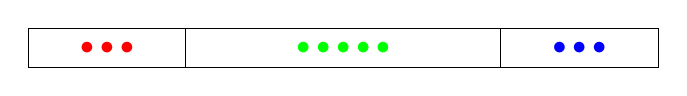
\begin{tikzpicture}
    \draw (0, 0) -- (8, 0);
    \draw (0, .5) -- (8, .5);
    \draw (0, 0) -- (0, .5);
    \draw (8, 0) -- (8, .5);
    \node[color=red] at (1, .25) {$\bullet\bullet\bullet$};
    \draw (2, 0) -- (2, .5);
    \node[color=green] at (4, .25) {$\bullet\bullet\bullet\bullet\bullet$};
    \draw (6, 0) -- (6, .5);
    \node[color=blue] at (7, .25) {$\bullet\bullet\bullet$};
\end{tikzpicture} 
\end{array} $$
which allows us to rely on tagging and pattern matching for composing and decomposing concatenations.

We propose that for shapes $\sigma, \dots$ and tags~$T, \dots$ we have a shape type $\sconcattype{T : \sigma, \dots}$ indexed by variants of type $\svarianttype{T : \sigma, \dots}$.
% Variants provide us with \textbf{concatenation} on array shapes.

\section{Calculus}
\label{sec:calculus}

\begin{figure}
    \centering
    \begin{align*}
\graintro e
n \mid f  
& \text{(integer and float literal)} 
\graitem
\pi(\overline{e}) 
& \text{(scalar operations)}
\graitem
x
\mid \slet{x}{e}{e}
& \text{(variable, let-binding)}
\graitem
\slam{x}{e}
\mid e\,e 
& \text{(function, application)}
\graitem
\srecordval{\overline{\ell = e}} 
& \text{(record construction)}
\graitem
\sproj{e}{\ell} 
& \text{(record projection)}
\graitem
\stag{T}{e} 
& \text{(variant construction)}
\graitem
\smatch{e}{\overline{\mid T\,x\,\Rightarrow e}} 
& \text{(pattern matching)}
\graitem
\sbuild{x}{e}{e} 
& \text{(array comprehension)}
\graitem
\sarrayval{s}{J} 
& \text{(unevaluated array)}
\graitem
\sindex{e}{e} 
& \text{(array indexing)}
\graitem
\sshape{e} 
& \text{(array shape)} 
\graitem
\eess
& \text{(shape expression)} 
\\ \\
% shape expressions
\graintro{\eess}
\ssize{e} 
& \text{(sized shape)}
\graitem
\sproductval{\overline{ \ell = e }} 
& \text{(product shape)} 
\graitem
\sproductproj{e}{\ell} 
& \text{(product dimension projection)}
\graitem
\sconcatval{\overline{ T = e }} & \text{(concatenation shape)}
\graitem
\sconcatproj{e}{T} 
& \text{(concatenation component projection)}
\graitem
\sbroadcast{e}{e} 
& \text{(shape broadcasting)}
\end{align*}
    \caption{Expressions $e$ in Star, including shape expressions $\eess$.}
    \label{fig:star-expressions}
\end{figure}

\begin{figure}
    \centering
    \begin{align*}
% \\ \\
% values
\graintro v
n \mid f   
& \text{(integer, float)}
\graitem
\slam{x}{e} 
& \text{(function)}
\graitem
\srecordval{\overline{\ell = v}} 
& \text{(record)} 
\graitem
\stag{T}{v} & \text{(variant)} \\ \mid&\,\,
\sarrayval{\vess}{I} & \text{(array)} \\ \mid&\,\,
\vess & \text{(shape value)} 
\\ \\
% shape values
\graintro{\vess}
\ssize{n} 
& \text{(sized shape)}
\graitem
\sproductval{\overline{ \ell = \vess }} 
& \text{(product shape)}
\graitem
\sconcatval{\overline{ T = \vess }} 
& \text{(concat. shape)}
\end{align*}
    \caption{Values $v$ in Star, including shape values $\vess$.}
    \label{fig:star-values}
\end{figure}

I now introduce the design of \textbf{Star} (\textbf{st}ructured \textbf{ar}rays), a functional, pointful array programming calculus with a novel type system. We begin by introducing expressions (Section~\ref{subsec:star-intro}) and our novel structured array shapes (Sections~\ref{subsec:array-shapes}~and~\ref{subsec:shape-bounds}) in Star.
Lastly, we give an operational semantics  (Section~\ref{subsec:semantics}).

\subsection{Introduction}
\label{subsec:star-intro}

The basis of Star is a $\lambda$-calculus with structurally typed records and variants. We define the grammars of expressions $e$ and values $v$ in Star in Figures~\ref{fig:star-expressions}~and~\ref{fig:star-values}.
We start with some informal explanations:

\begin{itemize}
    \item We write $\pi$ for scalar operations, which consume and produce integers and floats. Examples include $+: \sint \times \sint \sfntype \sint$, $\mathrm{sin} : \sfloat \sfntype \sfloat$, or $\lfloor \cdot \rfloor : \sfloat \sfntype \sint$.
    % \item Functions and let-bindings are standard. For simplicity, we do not include recursive let-bindings.
    \item We include structural records and variants, respectively introduced by construction $\srecordval{\overline{\ell = e}}$ and tagging $T\,e$, and eliminated with with projection $\sproj{e}{\ell}$ and pattern matching. 
    \item Star's array operations are similar to the likes of pointful calculi like $\tilde F$ \cite{f-smooth}. Our primitives are array comprehensions $\sbuild{x}{e}{e'}$ (constructing an array of shape $e$ and elements at index $x$ given by $e'$) and indexing $\sindex{e}{e'}$ (accessing index $e'$ of array $e$).
    The shape of an array $e$ is accessed by $\sshape{e}$.
\end{itemize}

\subsection{Array shapes}
\label{subsec:array-shapes}

The design of array shapes in Star -- both shape values here and shape types in Section~\ref{sec:typing} -- is a novel contribution.
In Star, array comprehensions require providing a shape.
We informally summarise them now and elaborate later. 
We have three constructors for shape values:
\begin{itemize}
    \item A sized shape $\ssize{e}$ is used for a usual flat array. For example, $\ssize{10}$ is the shape of an array indexed by integers in the range $[ 0, 10)$.
    \item Product shapes are used for defining arrays with multiple \textit{named} dimensions. For instance: 
    $$\sproductval{\mathrm{row} = \ssize{5}, \mathrm{col} = \ssize{4}}$$ 
    is the shape of a $5 \times 4$ matrix (with dimensions named as rows and columns). To index into an array of a product shape, we provide a record -- e.g.\@ $\srecordval{\mathrm{row} = 2, \mathrm{col} = 3}$.
    Products capture \textit{rectangular} (regular) multidimensional arrays.
    Note that an array of shape~$\sproductval{}$ has a single element.
    \item Concatenation shapes are given by a sequence of \textit{named} component shapes. For example,
    $$\sconcatval{ \mathrm{Left}= \sproductval{}, \mathrm{Centre}= \ssize{8}, \mathrm{Right}= \sproductval{} }$$
    describes an 8-element array with an extra element at the start and end (i.e.\ a halo/padding/boundary of size 1). We index into arrays of concatenation shapes with variants, e.g.\@ $\stag{\mathrm{Left}}{\srecordval{}}$ or $\stag{\mathrm{Centre}}{2}$.
    Note that an array of shape $\sconcatval{}$ is empty.
\end{itemize}
Projections on shapes extract dimensions/components of products/concatenations. For example: 
\begin{align*}
\sproductproj{ \sproductval{\mathrm{row} = \ssize{5}, \mathrm{col} = \ssize{4}}}{\mathrm{row}} &\step \ssize 5 \\
\sconcatproj{\sconcatval{ \mathrm{Left}= \ssize{1}, \mathrm{Right}= \ssize{0}}}{\mathrm{Left}} &\step \ssize 1
\end{align*}

\begin{figure}
    \centering
    \begin{align*}
\ssize{n} \broadcastsem \ssize{m} 
&= \ssize{n} 
& \text{if }n = m \\ 
% 
\sproductval{ \overline{\ell' = \vess_\ell'} } \broadcastsem \sproductval{ \overline{\ell'' = \vess_\ell''} } 
&= \sproductval{\overline{\ell = \vess_\ell' \broadcastsem \vess_\ell''} } 
& \text{for }\ell = \ell' \cup \ell'' \\
% 
\sconcatval{ \overline{T = s_T'} } \broadcastsem \sconcatval{ \overline{T = s_T''} } \ 
&= \sconcatval{ \overline{T = s_T' \broadcastsem s_T''} }
\end{align*}
    \caption{
        Semantics $\broadcastsem$ of shape broadcasting $\broadcast$. 
        We take the union of sets of dimensions $\ell$ (defaulting $s_\ell' = s_\ell''$ if either is absent), but equate sets of components $T$. 
        If $\vess' \broadcastsem \vess''$ is undefined, we say $\vess'$ and $\vess''$ are \emph{incompatible}, and $\sbroadcast{\vess'}{\vess''}$ is a stuck state in the operational semantics.
    }
    \label{fig:broadcasting}
\end{figure}

Lastly, Star's \textit{shape broadcasting}
operation $e \broadcast e'$ (see Figure \ref{fig:broadcasting}) is used to \textit{align} compatible shapes $e$ and $e'$ by finding their common \emph{sub-shape} (cf.\@ broadcasting in NumPy \cite{numpy}), so that, for example:
$$ \sproductval{\mathrm{row}: \ssized 5} \broadcast \sproductval{\mathrm{col}: \ssized 4} \text{ evaluates to } \sproductval{\mathrm{row}: \ssized 5, \mathrm{col}: \ssized 4}$$
The name sub-shape refers to the result having possibly more dimensions, paralleling subtyping.
% We define broadcasting precisely and elaborate on its uses in Section~\ref{subsec:shape-broadcasting}.

\subsection{Shape bounds}
\label{subsec:shape-bounds}

We now formalise what indices $v$ can be used to index into a given shape $s$ by using the \emph{in-bounds} relation $v \inbs s$, defined in Figure \ref{fig:in-bounds}.

For integers, in-bounds behaves as expected. 
However, structural indices have more interesting behaviour thanks to subtyping:
for products, an index with more dimensions than the shape can be used for indexing; for concatenations any component works. 
To manipulate these extra dimensions, we define a \emph{cast} operator $\scast{v}{s}$ in Figure~\ref{fig:cast}, which removes extra dimensions from $v$, coercing an index to fit the structure of a given shape exactly.
We then define the \emph{structurally-exact in-bounds} relation $v \inbsp s$ as:
$$ v \inbsp s \iff v \inbs s \text{ and } v = \scast{v}{s}$$
Lastly, we introduce a \emph{structurally-in-bounds} relation $v \inbstr \vess$, given by the same rules as $\inbs$ but with $n \inbstr \ssize m$ holding for \textbf{any} $n$ and $m$ (and not just $0 \le n < m$). We use this to state type safety later -- we only guarantee successful indexing up to integer indices.

Let us consider some examples. Both $\srecordval{ x = 3 } \inbs \sproductval{x = \ssize 4}$
and $\srecordval{ x = 3 } \inbsp \sproductval{x = \ssize 4}$ hold.
While we have $\srecordval{x = 3} \inbs \sproductval{}$, $\srecordval{x = 3} \inbsp \sproductval{}$ is false (since $\scast{\srecordval{x = 3}}{\sproductval{}} = \srecordval{}$) and only $\srecordval{} \inbsp \sproductval{}$ holds.

In the operational semantics, $\inbsp$ determines the indices $v$ for which we should compute and store the elements when building an array. $\scast{v}{s}$ is used instead of $v$ for indexing, but only when $v \inbs s$.

\begin{figure}
    \centering
    \begin{gather*}
\dfrac{}{n \inbs \ssize{m}} \quad \mbox{ if $0 \le n < m$} \\[1ex]
\dfrac{\forall \ell' \ldotp v_{\ell'} \inbs \vess_{\ell'}}{\srecordval{\overline{\ell = v_\ell}} \inbs
\sproductval{\overline{\ell' = \vess_{\ell'}}}} \qquad
\dfrac{v \inbs \vess_T}{T \, v \inbs \sconcatval{\overline{T = \vess_T}}}
\end{gather*}
    \caption{Definition of the in-bounds relation $v \inbs s$, stating that an index $v$ can be used to index into a shape $s$.}
    \label{fig:in-bounds}
\end{figure}

\begin{figure}
    \centering
    \begin{align*}
\scast{n}{\ssize{m}} &= n \\
\scast{
  \srecordval{\overline{\ell = v_\ell}, \overline{\ell' = v_\ell'}}}{
  \sproductval{\overline{\ell = s_\ell}}} &=
\srecordval{\overline{\ell = \scast{v_\ell}{s_\ell}}} \\
\scast{T\,v}{\sconcatval{\overline{T' = v_{T'}}}} &= T\,(\scast{v}{v_T})
\end{align*}
    \caption{Definition of the index-shape cast $\scast{v}{s}$, which removes dimensions from $v$ which do not appear in $s$.}
    \label{fig:cast}
\end{figure}

\subsection{Representation of array values}
\label{subsec:array-values}

In Star, array comprehensions $\sbuild{x}{e}{e'}$ eventually evaluate to array values $\sarrayval{\vess}{I}$.
These consist of a shape value $\vess$ along with a partial function (taken as a set) $I$ from index values to element values.
The domain of $I$ consists of exactly the indices $v$ which are within bounds of $s$: $v \inbsp s$.

However, evaluating  $\sbuild{x}{e}{e'}$ generally requires multiple evaluations of $e'$; our small-step operational semantics achieves this using \emph{unevaluated array expressions} $\sarrayval{\vess}{J}$.
These generalise array values above, allowing the codomain of $J$ to hold expressions instead of values.
Operationally, array comprehensions $\Phi$ yield array expressions $\sarrayval{s}{J}$, which are evaluated until they become values $\sarrayval{s}{I}$.
$\sarrayval{\vess}{J}$ is not part of the user-facing expression syntax -- it exists solely to enable a \emph{small-step} operational semantics, thus simplifying the statement and proofs of type safety.

\subsection{Semantics}
\label{subsec:semantics}

Finally, I present a call-by-value operational semantics for Star in Figure~\ref{fig:opsem} via a \emph{steps-to} relation $e \step e$.

Run-time errors (e.g.\@ out-of-bounds indexing)
manifest as \emph{stuck states}, which do not step further. Most stuck states are prevented by Star's type system -- for errors which are not, we introduce a \emph{raises-error} relation $e \sterr$ in Figure \ref{fig:opsem-err} (we use it to state type safety in Section \ref{subsec:type-safety}).

Successful executions eventually reduce to a value $v$ (Figure~\ref{fig:star-values}). 

\begin{figure}
    \centering
    \renewcommand\arraystretch{1.5}
\begin{gather*}
\boxed{e \sterr} \\[0.5em]
\begin{array}{rlr}
\sarrayval{\vess}{I}[v] 
\leadsto \lightning 
&\text{ if } (v \inbstr \vess) \land \lnot (v \inbs \vess) 
& \textsc{StepIndexErr} \\
\vess' \broadcast \vess'' 
\leadsto \lightning 
&\text{ if } \vess' \broadcastsem \vess'' \text{ is undefined} 
&\quad \textsc{StepBroadcastErr}
\end{array}
\\
\irule{CongErr}{e \leadsto \lightning}{\ctx{\evalct}{e} \leadsto \lightning}
\end{gather*}

    \caption{Raises-error step relation $e \sterr$, used for specifying errors which \emph{can} occur in well-typed Star programs.}
    \label{fig:opsem-err}
\end{figure}

\begin{figure}
    \centering
    \begin{align*}
\multispan{3}{\hfil$\displaystyle \boxed{e \step e}$\hfil} \\[1em]
% 
% 
(\slam{x}{e})\,v 
&\leadsto \subst{v}{x}{e} 
& \textsc{StepApply} \\ 
% 
\slet{x}{v}{e} 
&\leadsto \subst{v}{x}{e}
& \textsc{StepLet} \\ 
% 
\sproj{\srecordval{\overline{\ell = v_\ell}}}{\ell} &\leadsto v_\ell 
& \textsc{StepRecordProj} \\
% 
\smatch{\stag{T}{v}}{T\,x\Rightarrow e \mid \cdots} 
&\leadsto \subst{v}{x}{e}
& \textsc{StepMatch} \\
% 
% \dfrac{\forall v : v \inbs \vess \ldotp  \leadsto^* w_v}{
\sbuild{x}{\vess}{e} 
&\leadsto \sarrayval{\vess}{\{ v \mapsto \subst{v}{x}{e} \mid v \inbsp \vess \}} 
& \textsc{StepArray} \\
% 
\sindex{\sarrayval{\vess}{I}}{v} 
&\leadsto I(\scast{v}{s})\;\;\
\text{ (if $v \inbs \vess$)}
& \textsc{StepIndex} \\
% 
\sshape{\sarrayval{\vess}{I}} 
&\leadsto \vess 
& \textsc{StepShape} \\
% 
\sproductproj{\sproductval{\overline{\ell= v_\ell}}}{\ell} 
&\leadsto v_\ell
& \textsc{StepProductProj} \\
% 
\sconcatproj{\sconcatval{\overline{T = v_T}}}{T} 
&\leadsto v_T 
& \textsc{StepConcatProj} \\
% 
\vess' \broadcast \vess'' 
&\leadsto \vess' \broadcastsem \vess'' 
& \textsc{StepBroadcast} 
\\[0.5em]
% 
% 
\multispan{3}{\hfil$\displaystyle \irule{Cong}{e \leadsto e'}{\evalct{C}{e} \leadsto \evalct{C}{e'}}$\hfil}
\end{align*} 

    \caption{
        Small-step operational semantics for Star. We write $e \step e'$ when $e$ reduces to $e'$.
        Evaluation contexts $\evalctx$ are defined in Appendix \ref{extra:star-proofs} -- I remark that we never evaluate under $\lambda$ or $\Phi$; but we evaluate expressions in $\sarrayval{s}{J}$.
        Note that indexing and broadcasting may result in a \emph{stuck state}, and that if $v \inbs s$ holds, then $\scast v s$ is well-defined.
    }
    \label{fig:opsem}
\end{figure}

\section{Typing}
\label{sec:typing}

\begin{figure}[t]
    \centering
    \begin{align*}
\graintro \tau
\top \mid \bot 
& \text{(top, bottom)} 
\graitem
\mathrm{int} \mid \mathrm{float} 
& \text{(integer, float)}
\graitem
\tau \sfntype \tau 
& \text{(function)} 
\graitem
\srecordtype{\overline{\ell : \tau}} 
& \text{(record)} 
\graitem
\svarianttype{\overline{T : \tau}} 
& \text{(variant)}
\graitem
\sarraytype{\sigma_1}{\sigma_2}{\tau} \quad \text{for } \sigma_1 \sub \sigma_2 
& \text{(array)}
\graitem
\sigma 
& \text{(shape)} \\ 
\\
\graintro \sigma
\ssized 
& \text{(sized)}
\graitem
\sproducttype{\overline{ \ell : \sigma }} 
& \text{(product)} 
\graitem
\sconcattype{\overline{ T : \sigma }} 
& \text{(concatenation)} \\
\\
\graintro \eta
\mathrm{int} 
\mid
\srecordtype{\overline{\ell : \eta}} 
\mid
\svarianttype{\overline{T : \eta}} & \text{(indices in } \tau)
\end{align*}
    \caption{Types $\tau$ in Star, showing their subtypes: shape types $\sigma$
    and index types $\eta$.
    % Note that $\sigma$ and $\eta$ are in bijection (see Figure~\ref{fig:indices}).
    Array types $\sarraytype{\sigma_1}{\sigma_2}{\tau}$ are defined only when $\sigma_1 \sub \sigma_2$ (with $\sub$ as in Figure~\ref{fig:subtyping}) -- we elaborate in Section \ref{sec:typing}.
    }
    \label{fig:types}
\end{figure}

\begin{table}[t]
    \centering
    \begin{tabular}{@{}cc|cc@{}}
\multicolumn{2}{c|}{Shape} & \multicolumn{2}{c}{Index} \\
Type & Value & Type & Value \\ \hline
$\ssized$ & $\ssize{5}$ & $\sint$ & $4$ \\
$\sproducttype{ r : \ssized, c : \ssized }$ & $\sproductval{r = \ssize{5}, c = \ssize{4} }$ & $\srecordtype{ r : \sint, c : \sint }$ & $\srecordval{ r = 4, c = 3 }$ \\ 
$\sconcattype{L : \ssized, R : \ssized}$ & $\sproductval{ L = \ssize{10}, R = \ssize{20} }$ & $\svarianttype {L: \sint, R: \sint}$ & $\stag{R}{19}$ \\ 
\end{tabular}
    \caption{Examples of shapes and matching indices. Given a shape of type $\sigma$ on the left, we have an index of type $\iota(\sigma)$ on the right.}
    \label{tab:shape-index-examples}
\end{table}

We now move on to Star's type system, which features novel aspects, matching the design of structural shape and index types. 
I give a complete description of the type language in Figure~\ref{fig:types}, subtyping in Figure~\ref{fig:subtyping}, and the typing judgement in Figure~\ref{fig:typing}. 

I first focus on the typing of array shapes and indices.\todo[color=red]{records?}
Afterwards, I state type safety for Star in Section \ref{subsec:type-safety}, and show how to apply the type inference framework from Chapter \ref{algebraic-subtyping} to Star in Section~\ref{subsec:type-inference}.

% I use a standard presentation of record (and similar) types \cite{tapl} for Star, unlike FL (Chapter \ref{static-soul}).

\begin{figure}[p]
    \centering
    \renewcommand\arraystretch{1.3}
$$\boxed{\tau \sub \tau}$$
\vspace{-1.5em}
\small
$$ \begin{array}{c}
\irule{SubRefl}{}{\tau \sub \tau} \quad 
\irule{SubTrans}{\tau \sub \tau' \quad \tau' \sub \tau''}{\tau \sub \tau''} \quad
\irule{SubTop}{}{\tau \sub \top} \quad 
\irule{SubBot}{}{\bot \sub \tau} \quad 
\\
\irule{SubFun}{\tau_1' \sub \tau_1 \quad \tau_2 \sub \tau_2'}{(\tau_1 \sfntype \tau_2) \sub (\tau_1' \sfntype \tau_2')} \quad 
{
\irule{SubArray}{\sigma_1' \sub \sigma_1 \quad \sigma_2 \sub \sigma_2' \quad \tau \sub \tau'}{\sarraytype{\sigma_1}{\sigma_2}{\tau} \sub \sarraytype{\sigma_1'}{\sigma_2'}{\tau'}} } \\
\irule{SubRecWidth}{}{\srecordtype{\ell: \tau, \rho} \sub \srecordtype{\rho}} \;
\irule{SubRecDepth}{\tau \sub \tau'}{\srecordtype{\ell: \tau, \rho} \sub \srecordtype{\ell : \tau', \rho}} \quad 
\irule{SubProdWidth}{}{\sproducttype{\ell: \tau, \rho} \sub \sproducttype{\rho}} \;
\irule{SubProdDepth}{\tau \sub \tau'}{\sproducttype{\ell: \tau, \rho} \sub \sproducttype{\ell : \tau', \rho}} \\
\irule{SubVarWidth}{}{\svarianttype{\rho} \sub \svarianttype{T: \tau, \rho}} \;
\irule{SubVarDepth}{\tau \sub \tau'}{\svarianttype{T: \tau, \rho} \sub \svarianttype{T : \tau', \rho}} \quad 
\irule{SubConcatWidth}{}{\sconcattype{T: \tau, \rho} \sub \sconcattype{\rho}} \;
\irule{SubConcatDepth}{\tau \sub \tau'}{\sconcattype{T: \tau, \rho} \sub \sconcattype{T : \tau', \rho}} 
% \\
% \irule{SubShapeSize}{}{\ssized \sub \sigma} \,
% \irule{SubShapeProd}{\tau \sub \sigma \quad \sproducttype{\rho} \sub \sigma}{\sproducttype{\ell: \tau, \rho} \sub \sigma} \,
% \irule{SubShapeConcat}{\tau \sub \sigma \quad \sconcattype{\rho} \sub \sigma}{\sconcattype{T : \tau, \rho} \sub \sigma} \quad
% \irule{SubIndexInt}{}{\mathrm{int} \sub \eta} \,
% \irule{SubIndexRecord}{\tau \sub \eta \quad \sproducttype{\rho} \sub \eta}{\sproducttype{\ell : \tau, \rho} \sub \eta} \,
% \irule{SubIndexVariant}{\tau \sub \eta \quad \sconcattype{\rho} \sub \eta}{\sconcattype{T: \tau, \rho} \sub \eta}
\end{array} $$
    \caption{
        Subtyping relation $\tau \sub \tau$. \textsc{SubArray} is particularly noteworthy, as it mixes contravariance of indices and covariance of shape-access. 
        % We include rules for specifying $\sigma$ to be a supertype of shape types and $\eta$ a supertype of index types. 
        We write $\rho$ for a list of entries in a type (like fields of a record). 
    }
    \label{fig:subtyping}
\end{figure}
~
\begin{figure}[p]
    \centering
    \renewcommand\arraystretch{1.3}
$$\boxed{\Gamma \vdash e : \tau}$$
\vspace{-1em}
\small
$$ \begin{array}{c}
\Gamma ::= \cdot \mid \Gamma, x : \tau \\
% fundamentals
\irule{Sub}{\Gamma \vdash e : \tau \quad \tau \sub \tau'}{\Gamma \vdash e : \tau'} \quad
\irule{Var}{\Gamma(x) = \tau}{\Gamma \vdash x : \tau} \quad
\irule{Int}{}{\Gamma \vdash n:\mathrm{int}} \quad
\irule{Float}{}{\Gamma \vdash f:\mathrm{float}} \\
\irule{Let}
     {\Gamma \vdash e:\tau \quad \Gamma,x:\tau \vdash e':\tau'}
     {\Gamma \vdash \slet{x}{e}{e'} : \tau'} \quad
\irule{Lambda}{\Gamma,x:\tau \vdash e':\tau'}{\Gamma \vdash \slam{x}{e}: \tau\sfntype\tau'} \quad
\irule{Apply}{\Gamma \vdash e:\tau'\sfntype\tau \quad \Gamma \vdash e':\tau'}{\Gamma \vdash e \, e' : \tau} \\
% records
\irule{Record}
     {\forall \ell \ldotp \Gamma \vdash e_\ell:\tau_\ell}
     {\Gamma \vdash \srecordval{ \overline{\ell = e_\ell} } : \srecordtype{ \overline{ \ell : \tau_\ell } }} \!
\irule{RecordProj}{\Gamma \vdash e : \srecordtype{\ell : \tau} }{\Gamma \vdash \sproj{e}{\ell} : \tau} 
% variants
\irule{Tag}{\Gamma \vdash e : \tau}{\Gamma \vdash \stag{T}{e} : \svarianttype{T : \tau }} \!
\irule{Match}{\Gamma \vdash e : \svarianttype{\overline{T : \tau_T}} \; \Gamma, x_T {:} \tau_T \vdash e_T : \tau}{\Gamma \vdash \smatch{e}{\overline{\stag{T}{x_T} \Rightarrow e_T}} : \tau} \\
% arrays
\irule{Array}
     {\Gamma \vdash e:\sigma \quad \Gamma,x:\iota(\sigma) \vdash e':\tau}
     {\Gamma \vdash \sbuild{x}{e}{e'} : \suniarraytype{\sigma}\tau} \quad
 \irule{ArrayLit}{\Gamma \vdash \vess : \sigma \quad \forall (v \mapsto e) \in J \ldotp \Gamma \vdash v : \iota(\sigma) \text{ and } \Gamma \vdash e : \tau}{\Gamma \vdash \sarrayval{\vess}{J} : \suniarraytype{\sigma}{\tau}} \\
\irule{Index}
     {\Gamma \vdash e:\sarraytype{\sigma_1}{\sigma_2}{\tau} \quad \Gamma \vdash e':\iota \left( \sigma_1 \right)}
     {\Gamma \vdash e[e'] : \tau} \;
\irule{Shape}{\Gamma \vdash e:\sarraytype{\sigma_1}{\sigma_2}{\tau}}{\Gamma \vdash \sshape{e}: \sigma_2} \quad
\irule{Broadcast}{\Gamma \vdash e : \sigma \quad \Gamma \vdash e' : \sigma'}{\Gamma \vdash \sbroadcast{e}{e'} : \sigma \meet \sigma'} \quad
% shapes
\irule{Sized}{\Gamma \vdash e:\sint}{\Gamma \vdash \ssize{e} : \ssized} \\
\irule{Product}
     {\forall \ell \ldotp \Gamma \vdash e_\ell:\sigma_\ell}
     {\Gamma \vdash \sproductval{\overline{ \ell = e_\ell }} : \sproducttype{\overline{ \ell : \sigma_\ell }}} \;
\irule{ProductProj}{\Gamma \vdash e : \sproducttype{\ell : \sigma}}{\Gamma \vdash \sproductproj{e}{\ell} : \sigma} \quad
\irule{Concat}
     {\forall T \ldotp \Gamma \vdash e_T:\sigma_T}
     {\Gamma \vdash \sconcatval{\overline{ T = e_T }} : \sconcattype{\overline{ T : \sigma_T }}} \;
\irule{ConcatProj}{\Gamma \vdash e : \sconcattype{T : \sigma}}{\Gamma \vdash \sconcatproj{e}{T} : \sigma}
\end{array} $$
    \caption{Rules for the typing judgement $\Gamma \vdash e : \tau$ for Star expressions $e$. We use $\sigma$ for metavariables standing for shape types.
    % \AMcomment{$\tau?$}
    % \AMcomment{CONCAT rule has been `corrected'}
    Note $\iota$ in \textsc{Array} and \textsc{Index} maps shape types $\sigma$ into corresponding index types $\eta$. 
    Quantifiers $\forall \ell$/$\forall T$ stand for an expanded list of assumptions instantiated for all appropriate $\ell$/$T$.
    }
    \label{fig:typing}
\end{figure}

\paragraph{Shapes and indices}

Recall that in Section \ref{subsec:shape-bounds} we determined that integers index into sized shapes, records into product shapes, and variants into concatenation shapes. This happens both at the value- and type-level, with examples in Table \ref{tab:shape-index-examples}.

While in basic array type systems it is sufficient to presume that the type of a shape $\sigma$ and a matching index $\eta$ are the same, in Star this is clearly not the case. We thus use a $\iota$ metafunction on types (defined in Figure \ref{fig:iota}): given a shape type $\sigma$, $\eta = \iota(\sigma)$ is the supertype of all matching index types for $\sigma$.

Constructing $\iota$ is unsurprising -- similar concepts often arise when generalising array-like structures, e.g.\@ \textit{containers} \cite{containers} or Naperian (representable) functors, which \textcite{naperian-apl} has found useful for statically modelling certain patterns of array programming. To the author's knowledge, neither of these have yet led to the key ideas present in Star.

\begin{figure}
    \centering
    \begin{align*}
\iota(\ssized) &= \sint \\ 
\iota \left(\sproducttype{\overline{\ell : \sigma_\ell}} \right) &= \srecordtype{\overline{\ell : \iota(\sigma_\ell)}} \\
\iota \left(\sconcattype{\overline{T : \sigma_T}} \right) &= \svarianttype{\overline{T : \iota(\sigma_T)}}
\end{align*}
    \caption{Definition of the metafunction $\iota$, which given a shape type $\sigma$ gives the least upper bound $\eta = \iota(\sigma)$ on its index type.}
    \label{fig:iota}
\end{figure}

\paragraph{Splitting $\sigma$} Let us direct our attention to Star's array types, which have the syntax $\sarraytype{\sigma_1}{\sigma_2}{\tau}$ for $\sigma_1 \sub \sigma_2$. They are carefully constructed to provide \emph{useful} subtyping for array types, and follow a technique used by both \textcite{dolan-thesis} and \textcite{pottier-thesis} (which they use for typing mutable reference types). The crux is to split the shape $\sigma$ in $\sonebound{\sigma}\tau$ into a contravariant part $\sigma_1$ and covariant part $\sigma_2$, so that indexing uses $\sigma_1$, while accessing the shape returns a $\sigma_2$. With a simpler array type like $\sonebound{\sigma}\tau$ (which we write to abbreviate $\sarraytype{\sigma}{\sigma}{\tau}$) array types would have to be invariant.\todo[color=purple]{cite paper} Notice that by requiring $\sigma_1 \sub \sigma_2$ there is a $\sigma$ such that $\sigma_1 \sub \sigma \sub \sigma_2$: we have an \emph{actual} shape $\sigma$ into which we index with $\iota(\sigma_1) \sub \iota(\sigma)$, and when accessing the shape we only obtain one of type $\sigma_2 \super \sigma$.

\paragraph{Broadcasting}
Our presented subtyping order forms a distributive lattice, in line with algebraic subtyping. 
This allows us to view as a meet in the lattices of both shape bounds and their types. 
Indeed, $\vess' \broadcastsem \vess''$ (for shape values $\vess': \sigma'$, $\vess'' : \sigma''$ of types $\sigma', \sigma''$) is a partial operator that finds the shape $\vess : \sigma$ for which $\sigma = \sigma' \meet \sigma''$ (where $\meet$ is the meet on types agreeing with $\sub$), so that for any index $v$: 
$$ v \inbs \vess \iff v \inbs \vess' \text{ and } v \inbs \vess'' $$
Hence, $\broadcast$ is the meet in a lattice spanned by the unary predicate $\_ \inbs s$, and its result type takes the meet of shape types: clarifying how broadcasting finds sub-shapes, as defined in Section~\ref{subsec:array-shapes}.

\subsection{Type safety}
\label{subsec:type-safety}

To show my design of Star is well-behaved, I state and prove type safety for it in the form of theorems of Preservation and Progress (in the simply-typed case, as presented so far). In the statement of Progress we refer to $e \sterr$, which captures errors that can occur even for well-typed programs -- out-of-bounds \emph{integer} indexing and invalid broadcasting.

\begin{theorem}[Preservation]
    If \ $\Gamma \vdash e : \tau$ and $e \leadsto e'$, then $\Gamma \vdash e' : \tau$.
\end{theorem}
\begin{theorem}[Progress]
    If \ $\cdot \vdash e : \tau$, then either $e$ is a value, $e \leadsto e'$ for some $e'$, or $e \leadsto \lightning$.
\end{theorem}

I prove these theorems in Appendix \ref{extra:star-proofs}, but they follow straightforwardly by structural induction. The key lemma shows agreement between the subtyping relation $\sub$ and the structurally-in-bounds relation $\inbstr$.


\subsection{Type inference \& polymorphism}
\label{subsec:type-inference}

It turns out that Star's subtyping relation both forms a distributive lattice\todo{closure!}, and $\iota$ forms a type lattice isomorphism.
Thus, we can apply the type inference framework developed in Chapter \ref{algebraic-subtyping}. 

Though I do not give a complete description of a polymorphic Star calculus, I show a sketch of constraint generation for Star in Figure \ref{fig:star-type-constraints}.

Extending Star with polymorphism enables a \emph{shape-polymorphic} programming style -- a generalisation of rank polymorphism in existing literature \cite{automap, sac-tensor-comprehensions}. 
It is worth noting that shape polymorphism gives us index safety for free akin to \textcite{theorems-for-free} (modulo integer indices).

Let us consider an example of type inference in action. Given the expression:
$$ \color{red} \text{TODO: something with broadcasting?} $$
we would infer for it the type scheme:
$$ \text{TODO} $$

\begin{figure}
    \centering
    \begin{align*}
        \Huge \color{red} \texttt{T O D O}
    \end{align*}
    \caption{Constraint generation for the key constructs in Star in the developed type inference framework.}
    \label{fig:star-type-constraints}
\end{figure}

\section{Case study}

To display the features of Star and its elegance in expressing common array programming patterns, we consider a case study of an array program -- and contrast to similar systems.\todo{todo}

\begin{center}
    \color{red} Slightly expanded padding example, contrast to NumPy and Dex?
\end{center}

\section{Conclusions}

I have presented a novel design for an array programming calculus, emphasising the use of structural types for array shapes. 
Though I do not statically ensure bounds checking for \emph{integer} indices -- like dependent type systems -- I circumvent the problem by enabling the programmer to use richer structures for their arrays' shapes (and indices). 
Thanks to this approach, it is much easier to provide useful static types to common array programming patterns. 
My novel type system for Star fills the gap between dynamically and dependently typed array programming.